\documentclass{article}
\usepackage[utf8]{inputenc}
\usepackage{graphicx} % Required for inserting images
\usepackage{hyperref}
\usepackage{subcaption}
\usepackage{float}
\usepackage{tcolorbox}
\usepackage{amsmath}
\usepackage{amssymb}
\usepackage{listings}% http://ctan.org/pkg/listings}
\usepackage{algorithm}
\usepackage{algorithmic}
\usepackage[toc,page]{appendix}
%\usepackage[backend=biber]{biblatex}
\usepackage{multicol}
\usepackage{siunitx}
\usepackage{comment}
\usepackage{xcolor}
\usepackage{caption}
\usepackage{forest}
\usepackage{tikz}
\usetikzlibrary{shapes.geometric, arrows}


\tikzstyle{startstop} = [rectangle, rounded corners, 
minimum width=3cm, 
minimum height=1cm,
text centered, 
draw=black, 
fill=red!30]

\tikzstyle{io} = [trapezium, 
trapezium stretches=true, % A later addition
trapezium left angle=70, 
trapezium right angle=110, 
minimum width=3cm, 
minimum height=1cm, text centered, 
draw=black, fill=blue!30]

\tikzstyle{process} = [rectangle, 
minimum width=3cm, 
minimum height=1cm, 
text centered, 
text width=3cm, 
draw=black, 
fill=orange!30]

\tikzstyle{decision} = [diamond, 
minimum width=3cm, 
minimum height=1cm, 
text centered, 
draw=black, 
fill=green!30]
\tikzstyle{arrow} = [thick,->,>=stealth]

% To delete lstlisting caption "Listing x"
%\captionsetup[lstlisting]{labelformat=empty}

\lstdefinestyle{myStyle}{
    belowcaptionskip=1\baselineskip,
    breaklines=true,
    frame=none,
    numbers=none, 
    basicstyle=\footnotesize\ttfamily,
    keywordstyle=\bfseries\color{green!40!black},
    commentstyle=\itshape\color{purple!40!black},
    identifierstyle=\color{black},
    backgroundcolor=\color{white},
}

\lstdefinestyle{cypherStyle}{
    backgroundcolor=\color{white},   % choose the background color
    basicstyle=\footnotesize\ttfamily,        % the size of the fonts that are used for the code
    commentstyle=\itshape\color{purple!40!black},
    keywordstyle=\bfseries\color{green!40!black},
    breakatwhitespace=false,         % sets if automatic breaks should only happen at whitespace
    breaklines=true,                 % sets automatic line breaking
    captionpos=b,                    % sets the caption-position to bottom
    commentstyle=\color{gray},    % comment style
    deletekeywords={},            % if you want to delete keywords from the given language
    escapeinside={\%*}{*)},          % if you want to add LaTeX within your code
    extendedchars=true,              % lets you use non-ASCII characters; for 8-bits encodings only, does not work with UTF-8
    %firstnumber=1000,                % start line enumeration with line 1000
    frame=none,                    % adds a frame around the code
    keepspaces=true,                 % keeps spaces in text, useful for keeping indentation of code (possibly needs columns=flexible)
    language=SQL,                    % the language of the code
    morekeywords={*,IF, REQUIRE, FOR, IS, LOAD, CSV, WITH, HEADERS, MERGE, toFloat, toInteger, date},            % if you want to add more keywords to the set
    numbers=none,                    % where to put the line-numbers; possible values are (none, left, right)
    numbersep=5pt,                   % how far the line-numbers are from the code
    numberstyle=\tiny\color{mygray}, % the style that is used for the line-numbers
    rulecolor=\color{black},         % if not set, the frame-color may be changed on line-breaks within not-black text (e.g. comments (green here))
    showspaces=false,                % show spaces everywhere adding particular underscores; it overrides 'showstringspaces'
    showstringspaces=false,          % underline spaces within strings only
    showtabs=false,                  % show tabs within strings adding particular underscores
    stepnumber=1,                    % the step between two line-numbers. If it's 1, each line will be numbered
    stringstyle=\ttfamily,     % string literal style
    tabsize=2,                       % sets default tabsize to 2 spaces
}

%% Golang definition for listings
%% http://github.io/julienc91/lstlistings-golang
%%
\lstdefinelanguage{Golang}%
  {morekeywords=[1]{package,import,func,type,struct,return,defer,panic,%
     recover,select,var,const,iota,},%
   morekeywords=[2]{string,uint,uint8,uint16,uint32,uint64,int,int8,int16,%
     int32,int64,bool,float32,float64,complex64,complex128,byte,rune,uintptr,%
     error,interface},%
   morekeywords=[3]{map,slice,make,new,nil,len,cap,copy,close,true,false,%
     delete,append,real,imag,complex,chan,},%
   morekeywords=[4]{for,break,continue,range,go,goto,switch,case,fallthrough,if,%
     else,default,},%
   morekeywords=[5]{Println,Printf,Error,Print,},%
   sensitive=true,%
   morecomment=[l]{//},%
   morecomment=[s]{/*}{*/},%
   morestring=[b]',%
   morestring=[b]",%
   morestring=[s]{`}{`},%
}

\lstdefinestyle{golangStyle}{
    captionpos=b,              % sets the caption-position to bottom
    belowcaptionskip=1\baselineskip,
    breaklines=true,
    frame=none,
    numbers=none, 
    basicstyle=\footnotesize\ttfamily,
    keywordstyle=\bfseries\color{green!40!black},
    commentstyle=\itshape\color{purple!40!black},
    identifierstyle=\color{black},
    backgroundcolor=\color{white},
    language=Golang,
}


\title{TFM-FernandoMartín}
\author{Fernando Martín Canfrán}
\date{April 2024}

\begin{document}

\textcolor{gray}{
Regarding the data model, the new nature of data requires a de facto new database paradigm
-continuously evolving databases- where data can be both stable and volatile. Even though
evolving databases can be implemented according to any approach, graph databases seem
especially well suited here [1, 2]. Indeed, the natural way to process evolving graphs as streams
of edges gives insights on how to proceed in order to maintain dynamic graph databases. Hence,
we consider that a suitable data model is a continuously evolving data graph, a graph having
persistent (stable) as well as non persistent (volatile) relations. Stable relations correspond
to edges occurring in standard graph databases while volatile relations are edges arriving indata streams during a set time interval. Once this time interval is over, the relations are not
longer valid so that there is no need to store them in the (stable) graph database. However,
when required -as for further legal or auditing purposes- timestamped occurrences of volatile
relations can be kept in a log file. Volatile relations induce subgraphs that exist only while the
relations are still valid. Without loss of generality, in this work we consider property graphs
(PG) [3, 4] as the basic reference data model. As an example, Figure 1a depicts part of a schema
of a PG database where stable relations correspond to the data that a bank typically gathers
on its issued cards, ATMs (Automated Teller Machines) network, etc. Volatile relations model
the interaction between cards and ATM entities}


\textcolor{blue}{In the context of our work we could see the data we are considering to be both static and streaming data, as we are considering a bank system application that contains all the information related to it on the cards, clients\dots, and that it is receiving the streaming of transactions that happens on it.
More specifically, the static data can be thinked of the classical bank database data, that is, the data a bank typically gathers on its issued cards, clients, accounts, ATMs\dots. Whereas as the streaming data we can consider the transactions the clients of the bank produce with their cards on ATMs, PoS\dots that reach the bank system.
Therefore, due to this nature of the data, we consider a \emph{continuously evolving database} paradigm, where data can be both stable and volatile. Even though 
evolving databases can be implemented according to any approach, graph databases seem especially well suited here \textcolor{blue}{\cite{angles2008survey, kumar2015graph}}. 
% TODO: PONER REFERENCIAS
% TODO: PONER + RAZONES?
}


The property graph data model consists of two sub property graphs: a stable and a volatile property graph. On the one hand, the stable is composed of the static part of the data that a bank typically gathers such as information about its clients, cards, ATMs (Automated Teller Machines). 
On the other hand, the volatile property graph models the transaction operations, which defines the most frequent and reiterative kind of interaction between entities of the data model.\\
The main difference and the main reason for this separation is the semantics with which we intentionally define each of the subgraphs: the stable will be understood like a fixed static bank database, whereas the volatile will be understood as the data model to define the transactions, as continuous interactions between the entities of the model, which will not be permanently saved, but instead, only for a certain window of time under the mission of detecting anomalous bank operations. Note that we will only model the transaction interaction in the volatile subgraph, only letting them occur here.
This separation will allow us to have a really simple and light property graph schema single-centered on the transactions with the minimal needed information (mostly identifiers of the entities a transaction links) and another, the stable, acting as a traditional bank database schema, from which to obtain the information details of the entities.

\textcolor{gray}{Due to the confidential and private nature of bank data, it was
impossible to find a real bank dataset nor a real bank data model. Therefore, we devoloped our own proposal of a bank database model.}

\subsection{Design of the Data Model}

In what follows we describe the design of our data model as a Property Graph data model, divided into the stable and volatile property graphs.

\subsubsection{Stable Property Graph}\label{section:stable-pg}

We propose a simplified stable data model where the defined entities, relations and properties modeling the bank database are reduced to the essential ones (see Figure \ref{img:pg-stable-def}).
Although it is obvious that a real bank data model is way more complex than the one we propose, we believe that ours is relevant and representative enough and therefore sufficient for the purpose of our work. 

\begin{figure}[H]
  \centering
  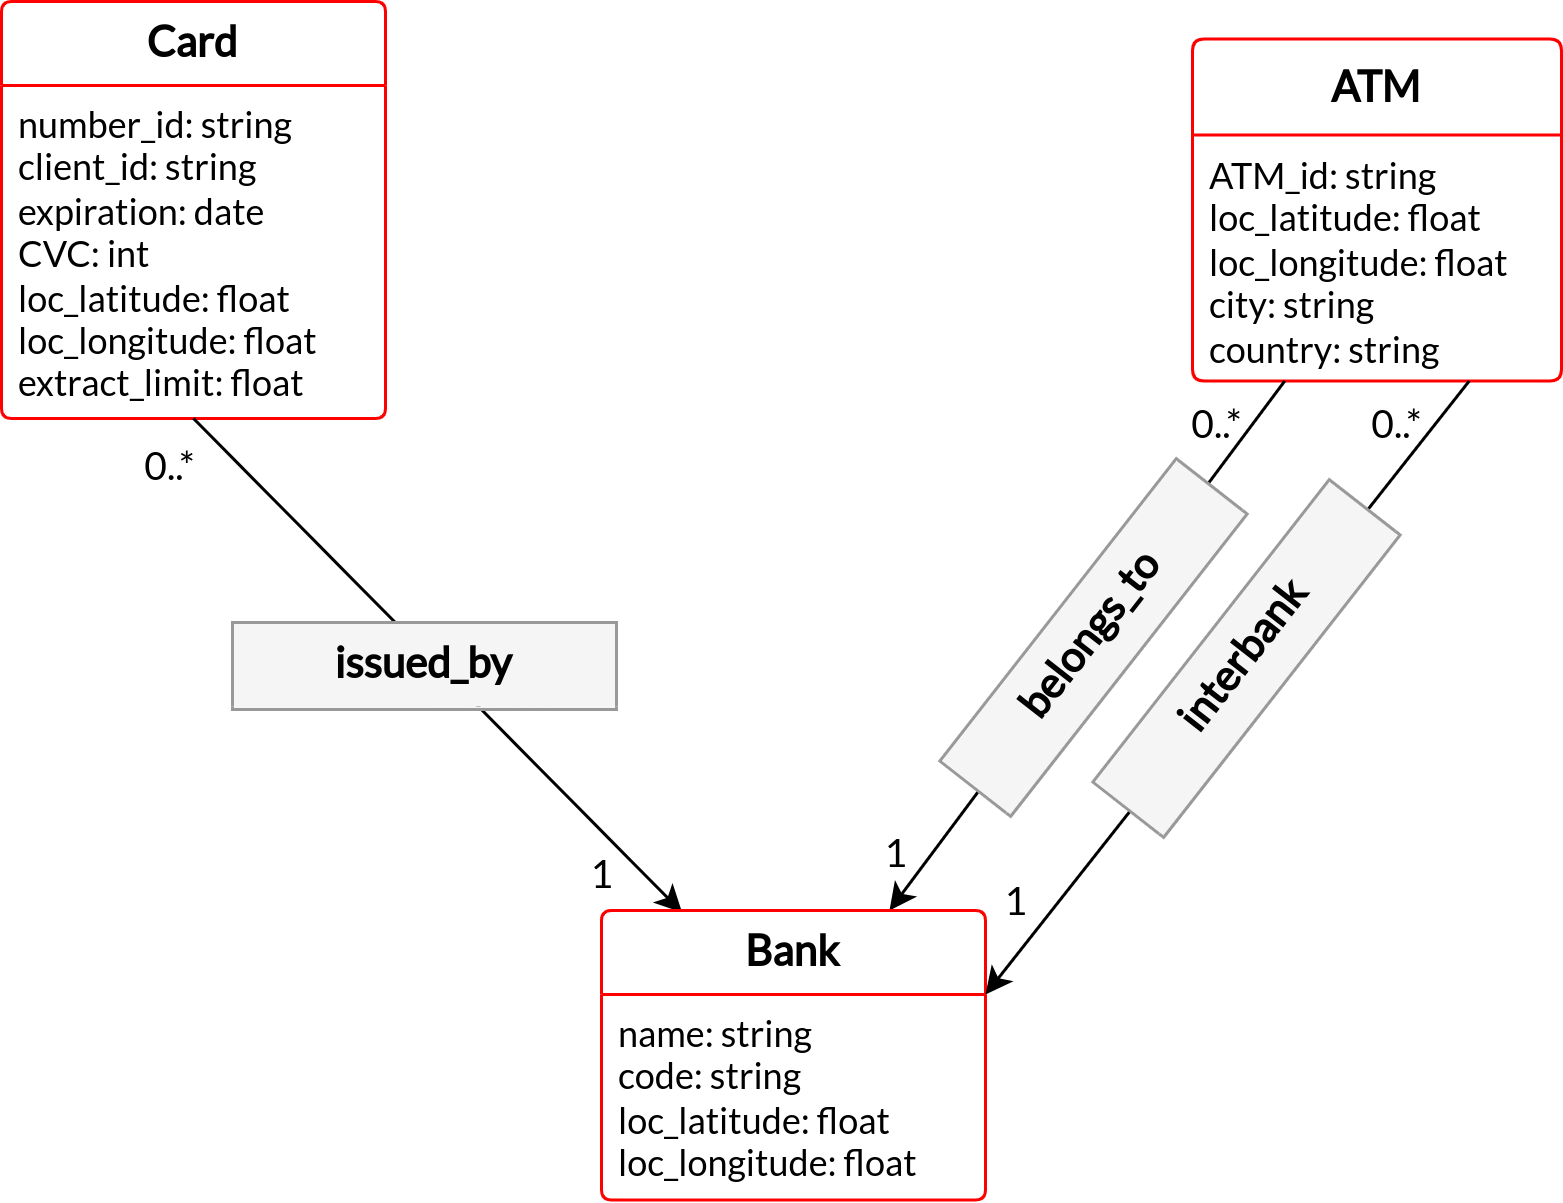
\includegraphics[scale = 0.7]{images/PG-stable-1-edit-cardinal.png}
  \caption{Definitive stable property graph model}
  \label{img:pg-stable-def}
\end{figure}

Before obtaining this final model, a first model proposal was developed (see Figure \ref{img:initial-pg-stable}), and then from it, we ended up reaching the final model version.\\

The first model idea was the initial attempt to capture the data that a bank system database typically gathers.
It contains four entities: Bank, ATM, Client and Card with their respective properties, and the corresponding relationships between them.

\begin{figure}[H]
  \centering
  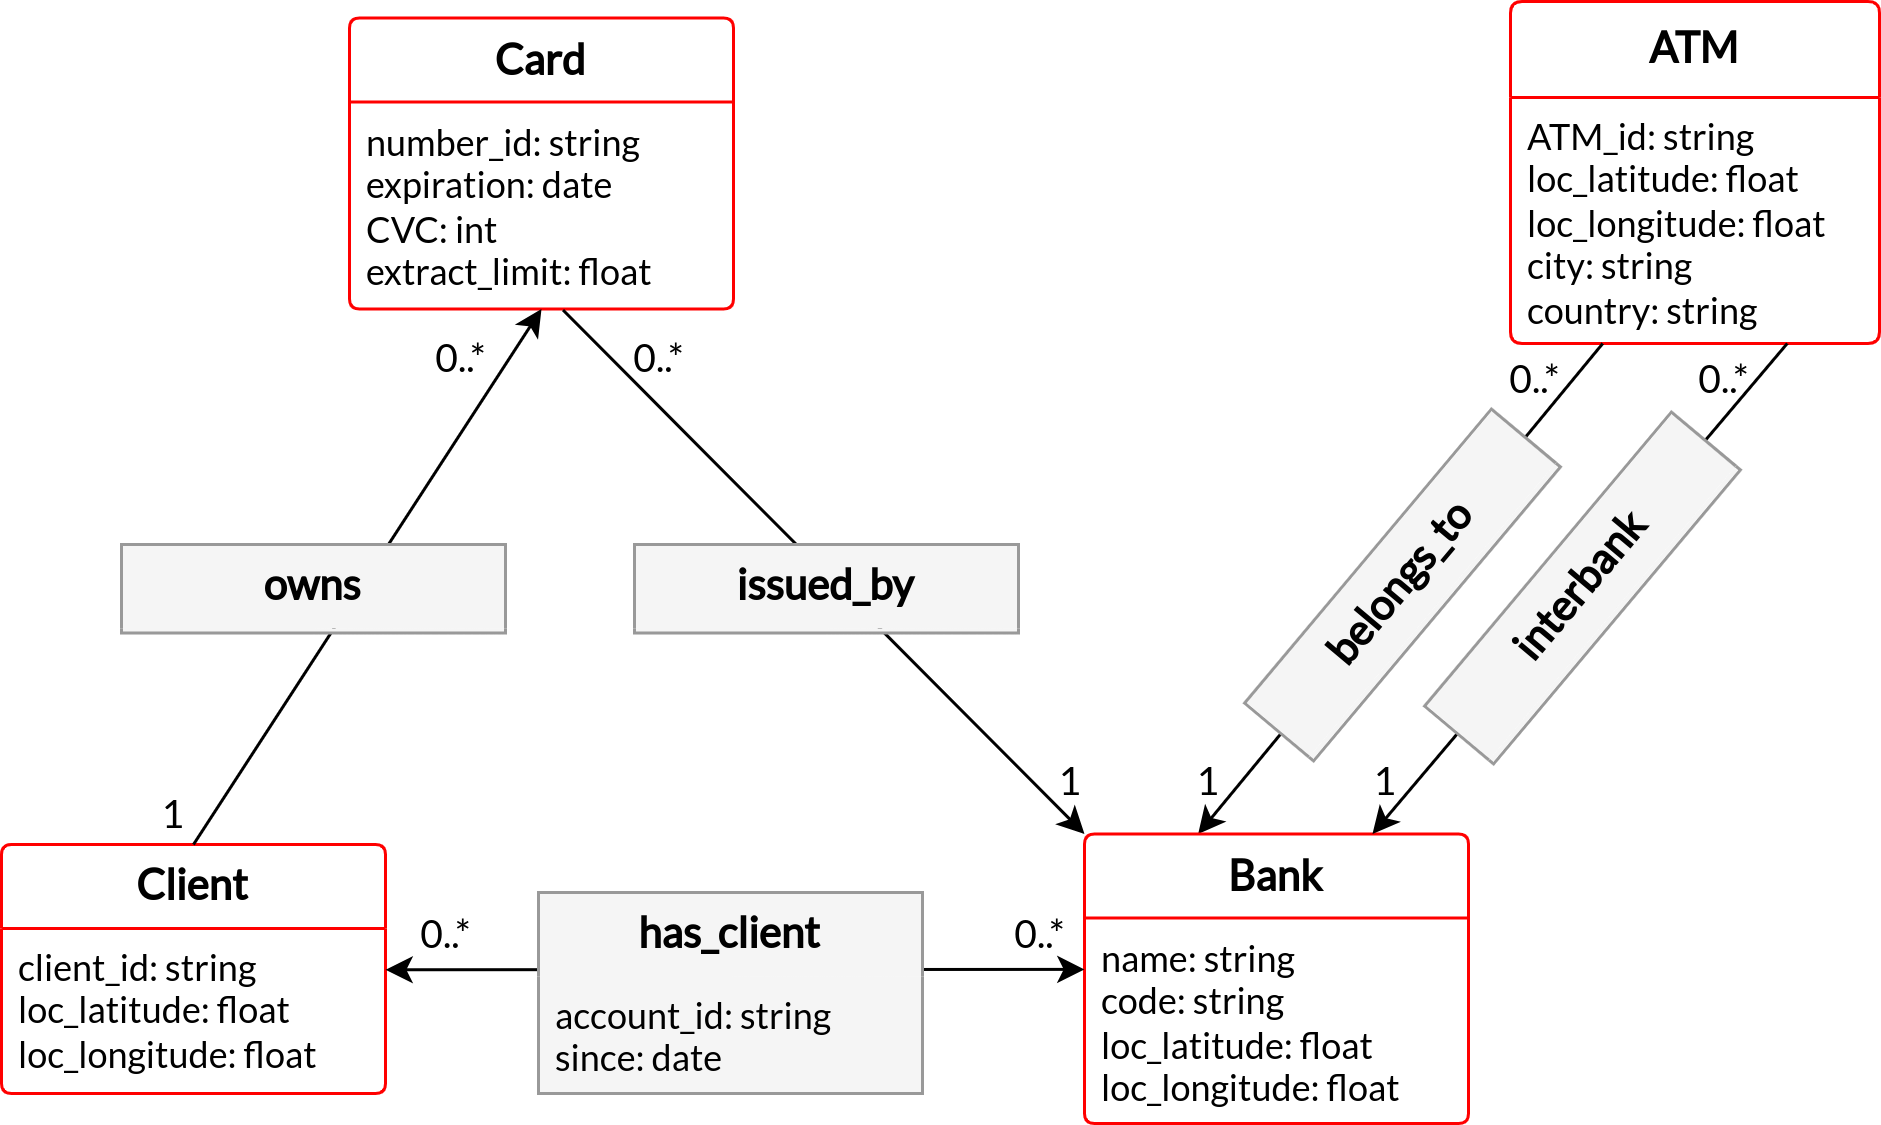
\includegraphics[scale = 0.7]{images/PG-stable-edit-cardinal.png}
  \caption{Initial bank stable property graph model}
  \label{img:initial-pg-stable}
\end{figure}

The relations are: a directed relationship from Client to Card \texttt{owns} representing that a client can own multiple credit cards and that a card is owned by a unique client, then a bidirectional relation \texttt{has\_client} between Client and Bank; representing bank accounts of the clients in the bank. The relation between Card and Bank to represent that a card is \texttt{issued\_by} the bank, and that the bank can have multiple cards issued. Finally, the relations \texttt{belongs\_to} and \texttt{interbank} between the ATM and Bank entities, representing the two different kinds of ATMs depending on their relation with the bank; those ATMs owned and operated by the bank and those that, while not owned by the bank, are still accesible for the bank customers to perform transactions.

However, the final version of the model (Figure \ref{img:pg-stable-def}) was simplified to reduce it to the minimal needed entities. In particular, we decided to remove the Client entity and to merge it inside the Card entity. For this, all the Client properties were included in the Card entity. In the initial schema the Client entity was defined with three properties: the identifier of the client and the GPS coordinates representing the usual residence of the client. This change is done while preserving the restriction of a Card belonging to a unique client the same way it was previously done with the relation between Card and Client \texttt{owns} in the initial schema, which now is therefore removed. \\
% Account relation removed
Another derived consequence of this simplification is the removal of the other relation that the Client entity had with other entities: the \texttt{has\_client} relation between Client and Bank, which was originally made with the intention of representing the bank accounts between clients and banks. Maintaining a bank account would imply having to consistently update the bank account state after each transaction of a client, complicating the model. Nevertheless, we eliminate the bank account relation, since its removal is considered negligible and at the same time helpful for the simplification of the model needed for the purposes of our work. % Properties included with the purpose of detecting frauds 
However, for the sake of completeness the property \textit{extract\_limit} is introduced in the Card entity, representing a money amount limit a person can extract, which will be related with the amount of money a person owns. This will allow the detection of anomalies related with frequent or very high expenses. Other properties that are included with the purpose to allow the detection of some other kinds of anomalies are the GPS coordinates, which are added intentionally in the case of the ATM and Card entities, in the first case referring to the geolocation of each specific ATM and in the last case referring to each specific client address geolocation. 

As a result, our stable property graph model contains three node entities: Bank, Card and ATM, and three relations: \texttt{issued\_by} associating Card entities with the Bank entity, and \texttt{belongs\_to} and \texttt{interbank} associating the ATM entities with the Bank entity. 

The Bank entitity represents the bank we are considering in our system. Its properties consist
on the bank \emph{name}, its identifier \emph{code} and the location
of the bank headquarters, expressed in terms of \emph{latitude} and \emph{longitude}
coordinates, as seen in Table \ref{table:bank-node-properties}.
  
\begin{table}[H]
    \centering
      \begin{tabular}{|l|l|}
      \hline
      \textbf{Name}        & \textbf{Description and value}                                      \\ \hline
      \texttt{name}         & Bank name                                                 \\ \hline
      \texttt{code}         & Bank identifier code                                      \\ \hline
      \texttt{loc\_latitude}  & Bank headquarters GPS-location latitude                   \\ \hline
      \texttt{loc\_longitude} & Bank headquarters GPS-location longitude                  \\ \hline
      \end{tabular}
    \caption{Bank node properties}
    \label{table:bank-node-properties}
\end{table}

\begin{tcolorbox}
\textcolor{red}{Note that, from the begining we were considering more than 1 bank entity. This lead to consider the creation of this entitity, which now as only 1 bank is considered it may not be needed anymore, being able to reformulate and simplify the model. However, it is left since we considered it appropiate to be able to model the different kinds of ATMs a bank can have with different relation types instead of with different ATM types.}
\end{tcolorbox}

The ATM entitity represents the Automated Teller Machines (ATM) that either belong to the bank's network or that the bank can interact with.
% Potential possible generalization of the ATM entity to a POS entity
For the moment, this entity is understood as the classic ATM, however note that this entity could potentially be generalized to a Point Of Sale (POS), allowing a more general kind of interactions apart from the current Card-ATM interaction, where also online transactions could be included apart from the physical ones. We distinguish two different kinds of ATMs, depending on their relation with the bank:

\begin{itemize}
  \item Internal ATMs: ATMs owned and operated by the bank. They are fully integrated within the
  bank's network. Modeled with the \texttt{belongs\_to} relation.
  \item External ATMs: These ATMs, while not owned by the bank, are still accessible for the bank
  customers to perform transactions. Modeled with the \texttt{interbank} relation. 
\end{itemize}

Both types of ATMs are considered to be of the same type of ATM node. Their difference
is modeled as their relation with the bank instance: \texttt{belongs\_to} for the internal ATMs and \texttt{interbank} for the external ATMs.

\begin{table}[H]
    \centering
    \begin{tabular}{|l|l|}
    \hline
    \textbf{Property}        & \textbf{Description}                                      \\ \hline
    \texttt{ATM\_id}      & ATM unique identifier                             \\ \hline
    \texttt{loc\_latitude}  & ATM GPS-location latitude           \\ \hline
    \texttt{loc\_longitude} & ATM GPS-location longitude          \\ \hline
    \texttt{city}         & ATM city location                         \\ \hline
    \texttt{country}      & ATM country location                       \\ \hline
    \end{tabular}
    \caption{ATM node properties}
    \label{table:atm-node-properties}
\end{table}

The ATM node type properties consist on the ATM unique identifier \emph{ATM\_id}, its location, expressed in terms of \emph{latitude} and \emph{longitude} coordinates, and the \emph{city} and 
\emph{country} in which it is located, as seen in Table \ref{table:atm-node-properties}.
Note that the last two properties are somehow redundant, considering that location coordinates
are already included. In any case both properties are maintained since their inclusion provides a more explicit description of the location of the ATMs.\\

Finally, the Card node type represents the cards of the clients in the bank system. The Card node type properties, as depicted in Table
\ref{table:card-node-properties}, consist on the card unique 
identifier \emph{number\_id}, the associated client unique identifier \emph{client\_id}, as well
as the coordinates of the associated client habitual residence address \emph{loc\_latitude} and 
\emph{loc\_longitude}. Additionally it contains the card validity expiration date \emph{expiration}, the Card Verification Code, \emph{CVC} and the \emph{extract\_limit} property, which represents the limit on the amount of money it can be extracted with the card on a single withdrawal.

\begin{table}[H]
    \centering
    \begin{tabular}{|l|l|}
    \hline
    \textbf{Name}        & \textbf{Description and value}                                          \\ \hline
    \texttt{number\_id}   & Card unique identifier                               \\ \hline
    \texttt{client\_id}   & Client unique identifier                               \\ \hline
    \texttt{expiration}   & Card validity expiration date                      \\ \hline
    \texttt{CVC}          & Card Verification Code                                      \\ \hline
    \texttt{extract\_limit} & Card money amount extraction limit    \\ \hline
    \texttt{loc\_latitude}  & Client's habitual address GPS-location latitude                         \\ \hline
    \texttt{loc\_longitude} & Client's habitual address GPS-location longitude                        \\ \hline
    \end{tabular}
    \caption{Card node properties}
    \label{table:card-node-properties}
\end{table}

The client is completely anonymized in the system (no name, surname, age, or any other confidential details) by using only a \emph{client\_id}. Currently, \emph{client\_id} is included in the Card node type for completeness. However, it could be omitted for simplicity, as we assume a one-to-one relationship between card and client for the purposes of our work -- each card is uniquely associated with a single client, and each client holds only one card. Thus, the \emph{client\_id} is not essential at this stage but is retained in case the database model is expanded to support clients with multiple cards or cards shared among different clients.

\textcolor{red}{$\Rightarrow ?$ Include in the card properties the properties related with the
gathered behavior for the card: \emph{withdrawal\_day}, \emph{transfer\_day}, 
\emph{withdrawal\_avg}... or just in the CSV to use them for the creation of the synthetic
transactions, but do not store them in the stable bank database}.


\textcolor{gray}{
Finally, as some remarks to complete the description, note that for both the ATM and the Card entities we have the GPS coordinates information. In the first case referring to the geolocation of each specific ATM and in the last case referring to each specific client address geolocation. These are included since they are needed for some of the transactions potential frauds that we want to detect.
Another property that was intentionally included with this purpose is the \texttt{extract\_limit} property on the Card node entity, it represents the money amount limit a person can extract, which will be related with the amount of money a person owns.This will allow the detection of anomalies related with frequent or very high expenses. 
}

\subsubsection{Volatile Property Graph}\label{section:volatile-pg}

The volatile subgraph model describes the most \emph{variable} part of our model, the continuous interactions between the client's cards and the ATMs. These interactions represent the transactions that are continuously occurring and arrive to our system as a continuous data stream. 
This subgraph model contains the minimal information needed to identify the Card and ATM entities -- \texttt{number\_id} and \texttt{ATM\_id} Card and ATM identifiers -- between which the interaction occurs, along with additional details related to the interaction. 
The proposed data model can be seen in the Figure \ref{img:pg-volatile}. On it we define the Card and ATM node entities with only the identifier properties, \texttt{number\_id} and \texttt{ATM\_id}, respectively. These identifiers are enough to be able to recover, if needed, the whole information about the specific Card or ATM entity in the stable subgraph.
Finally we define the \emph{interaction} relationship between the Card and the ATM nodes.
The \emph{interaction} relation contains as properties: \texttt{id} as the interaction unique identifier, \texttt{type} which describes the type of the interaction (withdrawal, deposit, balance inquiry or transfer), \texttt{amount} describing the amount of money involved in the interaction in the local currency considered, and finally, \texttt{start} and \texttt{end} which define the interaction \emph{datetime} start and end moments, respectively.

\begin{figure}[h]
    \centering
    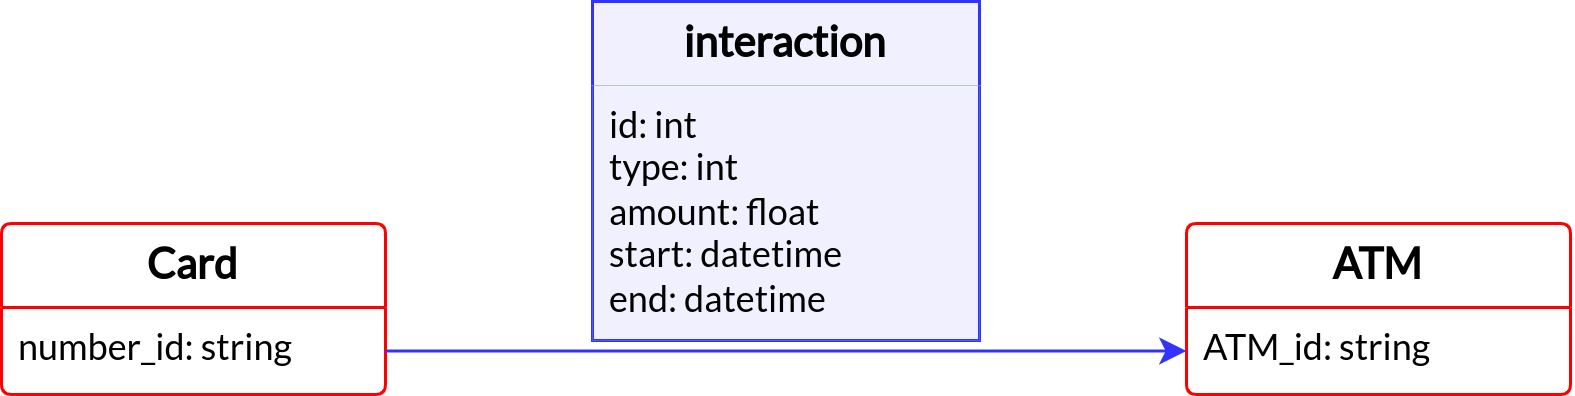
\includegraphics[scale = 0.8]{images/schema-volatile.png}
    \caption{Volatile property graph model}
    \label{img:pg-volatile}
\end{figure}


As a whole, the proposed property graph data model is represented in Figure \ref{img:pg-complete}. where both the stable and volatile property subgraphs are merged to give a full view on the final property graph model.

\begin{figure}[H]
  \centering
  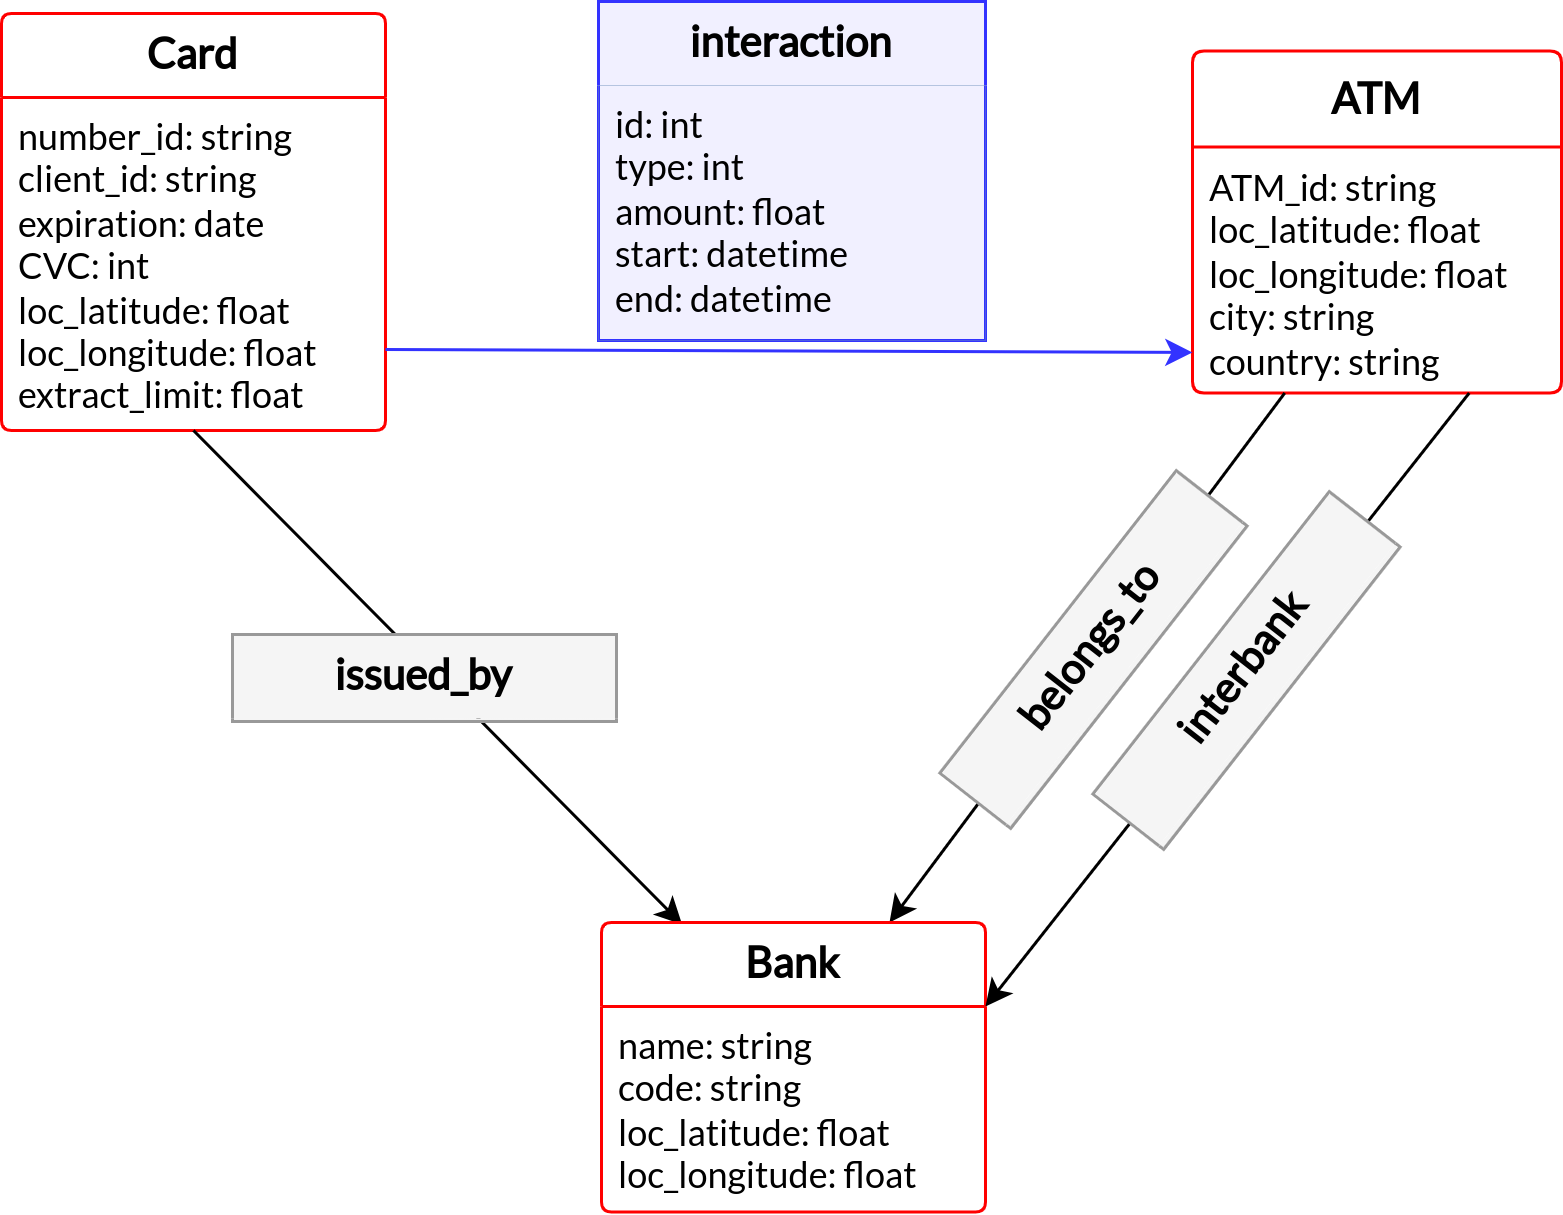
\includegraphics[scale = 0.7]{images/schema-complete.png}
  \caption{Complete property graph model}
  \label{img:pg-complete}
\end{figure}

\subsection{Creation of the Synthetic Dataset}

As mentioned, given the confidential and private nature of bank data, it was not possible to find any real bank datasets. In this regard, and based on the described data model, we built a synthetic dataset consisting on a stable property graph bank database and a set of volatile interactions (transactions).
For this we used the \emph{Wisabi Bank Dataset}\footnote{\href{https://www.kaggle.com/datasets/obinnaiheanachor/wisabi-bank-dataset}{Wisabi bank dataset on kaggle}} as a base to do the generation of the synthetic dataset. The \emph{Wisabi Bank Dataset} is a fictional banking dataset that was made publicly available in the Kaggle platform. We considered it of interest as a base for the synthetic bank
database that we wanted to develop. The interest to use this bank dataset as a base was mainly because of its size: it contains 8819 different customers, 50 different ATM locations and 2143838 transactions records of the different customers during a full year (2022). Additionally, it provides good heterogenity on the different kind of transactions: withdrawals, deposits, balance inquiries and transfers. The main uses of this bank dataset are the obtention of a geographical distribution for
the locations of our generated ATMs and the construction of a card/client \emph{behavior}, which we will use for the generation of the synthetic transactions.

In particular, we divide the creation of the synthetic dataset in two. On the one hand on the creation of the stable bank database and on the other hand on the creation of the set of synthetic transactions and anomalous transactions that will conform the stream of data reaching our system.

\paragraph{Details of the \emph{Wisabi Bank Dataset\\}}
The \emph{Wisabi Bank Dataset} consists on ten CSV tables. Five of them are of transaction records of five different states of Nigeria (Federal Capital Territory, Lagos, Kano, Enugu and Rivers State) that refers to transactions of cardholders in ATMs. In particular they contain 2143838 transactions records done during the year 2022, of which 350251 are in Enugu, 159652 in Federal Capital Territory, 458764 in Kano, 755073 in Lagos and 420098 in Rivers. Then, the rest of the tables are: a customers table (`customers\_lookup`) where the data
of 8819 different cardholders is gathered, an ATM table (`atm\_location lookup`) with
information of each of the 50 different locations of the ATMs, and then three remaining
tables as complement of the previous ones (`calendar lookup`, `hour lookup` and 
`transaction\_type lookup`) 
(\href{https://app.diagrams.net/#G1eAn47YR7-zPNE5KgStkA6_IJcxZRYgX8#%7B%22pageId%22%3A%22R2lEEEUBdFMjLlhIrx00%22%7D}{tables summary}).

\subsubsection{Stable Bank Database}

To do the generation of a stable bank database we provide the Python program \texttt{bankDataGenerator.py}, in which it is needed to enter the bank properties' values, 
as well as the parameters on the number of the bank ATMs (internal and external) and Cards: \texttt{n} and \texttt{m}, respectively. In what follows we give the details on the generation of the instances of our static database entities.
For simplicity and to do it in a more stepwise manner, we are going to first create all the CSV data tables for the nodes and for the relations in the corresponding format and then we will populate the Neo4j GDB with them.

\paragraph{Bank}

Since a unique bank instance is considered, the values of the properties of the bank node are manually assigned, leaving them completely customisable.
For the bank, we will generate \texttt{n} ATM and \texttt{m} Card entities. Note that apart from the generation of the ATM and Card node types we will also need to generate the relationships between the ATM and Bank entities (\texttt{belongs\_to} and \texttt{external}) and the Card and Bank entities (\texttt{issued\_by}).

\paragraph{ATM}

We generate $\texttt{n = n\_internal + n\_external}$ ATMs, where \texttt{n\_internal} is the number of internal ATMs owned by the bank and \texttt{n\_external} is the number of external ATMs that are accesible to the bank.
The generation of \texttt{n} ATMs for the bank is done following
the geographical distribution of the locations of the ATMs in the \emph{Wisabi Bank Dataset}. 
On this dataset there are 50 ATMs locations distributed along Nigerian cities. 
Note that for each of these ATMs locations, there can be more than one ATM.
However, this is not taken into account and only one ATM per location is assumed for the 
distribution.\\
\textcolor{red}{$\Rightarrow$ Put a plot of the distribution of the ATM locations}\\
This distribution of the ATMs matches the relevance of the location in terms of its population, since the number of ATM locations is larger in the most populated 
Nigerian cities (30\% of the ATM locations are in the city of Lagos, then the 20\% in Kano...). Therefore, for the generation of the location of each of the \texttt{n} ATMs, the location/city of an ATM selected uniformly at random from the \emph{Wisabi Bank Dataset} is assigned as \emph{city} and \emph{country}. Then, new random geolocation coordinates inside a bounding box of this city location are set as the \emph{loc\_latitude} and \emph{loc\_longitude} exact coordinates of the ATM. \\
Finally, as the ATM unique identifier \emph{ATM\_id} it is assigned a different code depending on the ATM internal or external category: 

\[
\emph{ATM\_id} =
\begin{cases} 
bank\_code + "-" + i & 0 \leq i < \texttt{n\_internal } \text{if internal ATM}  \\
EXT + "-" + i & 0 \leq i < \texttt{n\_external } \text{if external ATM}
\end{cases}
\]

\paragraph*{Card}

We generate a total of \texttt{m} cards that the bank manages, for each of them the assignment of the different properties is done as follows:

\begin{itemize}
\item Card and client identifiers:

\[
\begin{cases} 
number\_id = \text{c-}bank\_code\text{-}i \\
client\_id = i 
\end{cases}
0 \leq i < \texttt{m}
\]

\item \texttt{Expiration} and \texttt{CVC} properties: they are not relevant, could be empty 
  value properties indeed or a same toy value for all the cards. For completeness the  
  same values are given for all the cards: $\texttt{Expiration} = \text{2050-01-17}$, $\texttt{CVC} = 999$.

\item Client's habitual address location (\texttt{loc\_latitude}, \texttt{loc\_longitude}): two possible options were designed to define the client habitual residence address. In both 
cases they are random 
coordinates drawn from a bounding box of a location/city. The difference is on how the selection of the location/city is done:

  \begin{enumerate}
      \item Wisabi customers selection: Take the city/location of the habitual ATM of a random selected \emph{Wisabi} database customer. Note that in the \emph{Wisabi Bank Dataset} customers contain an identifier
      of their usual ATM, more in particular, the dataset is designed in such a way that customers
      only perform operations in the same ATM.
      With this approach, we maintain the geographical distribution of the \emph{Wisabi} customers.
      \item Generated ATMs selection: Take the city/location of a random ATM of the \texttt{n} generated ATMs. This method is the one utilized so far.
  \end{enumerate}

\item[$\circ$]\textbf{\emph{Behavior}}: It contains relevant attributes that will be of special interest when performing the 
generation of the synthetic transactions of each of the cards. The defined \emph{behavior}
parameters are shown in Table \ref{table:behavior-parameters}. 

\begin{table}[H]
    \centering
    \begin{tabular}{|l|l|}
        \hline
        \textbf{Behavior Property} & \textbf{Description} \\ 
        \hline
        $\mathsf{amount\_avg\_withdrawal}$ & Withdrawal amount mean\\ 
        \hline
        $\mathsf{amount\_std\_withdrawal}$ & Withdrawal amount standard deviation \\ 
        \hline
        $\mathsf{amount\_avg\_deposit}$ & Deposit amount mean \\ 
        \hline
        $\mathsf{amount\_std\_deposit}$ & Deposit amount standard deviation\\ 
        \hline
        $\mathsf{amount\_avg\_transfer}$ & Transfer amount mean \\ 
        \hline
        $\mathsf{amount\_std\_transfer}$ & Transfer amount standard deviation \\ 
        \hline
        $\mathsf{withdrawal\_day}$ & Average number of withdrawal operations per day \\ 
        \hline
        $\mathsf{deposit\_day}$ & Average number of deposit operations per day \\ 
        \hline
        $\mathsf{transfer\_day}$ & Average number of transfer operations per day \\ 
        \hline
        $\mathsf{inquiry\_day}$ & Average number of inquiry operations per day \\ 
        \hline
    \end{tabular}
    \caption{\emph{Behavior} properties}
    \label{table:behavior-properties}
\end{table}


For each card, its \emph{behavior} parameters are gathered from the transactions record of a randomly selected customer on the \emph{Wisabi Bank Dataset}, from which we can access the transactions record of $8819$ different customers for one year time interval. On it, there are four different types of operations that a customer can perform: withdrawal, deposit, balance inquiry and transaction. The parameters for the \emph{behavior} gather information about these four different types of operations. Note that all these \emph{behavior} parameters are added as additional fields of the CSV generated card instances, so, as mentioned, they can later be utilized for the generation of the synthetic
transactions.

Another possible way to assign the \emph{behavior} parameters could be the assignation
of the same behavior to all of the card instances. However, this method will provide less variability in
the generation of the synthetic transactions than the aforementioned method. 
Nevertheless, other taylored generation methods to generate different \emph{behavior} for 
each the cards could also be considered to similarly obtain this
variability.

\item \textcolor{red}{\texttt{extract\_limit}: $\texttt{amount\_avg\_withdrawal} * 5$} Other possible ways could be chosen for assigning a value to this property.
\end{itemize}

\subsubsection{Transactions Set}

\begin{comment}
\begin{itemize}
  \item[-] transaction\_id: Unique identifier for each transaction in the database.
  \item[-] transaction\_start: Datetime when the transaction started. Format: DD/MM/YYYY HH:MM (ex. 1/1/2022 4:50).
  \item[-] transaction\_end: Datetime when the transaction was completed. Format: DD/MM/YYYY HH:MM (ex. 1/1/2022 4:54).
  \item[-] transaction\_amount: Amount of money involved in the transaction.
\end{itemize}

\begin{figure}[H]
    \centering
    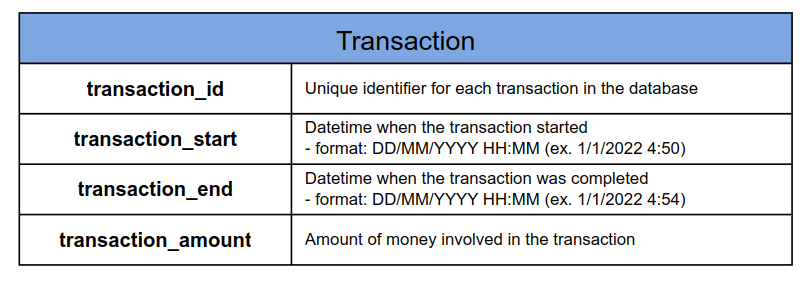
\includegraphics[scale = 0.40]{images/transaction.png}
    \caption{Transaction relation attributes}
    \label{img:pg-stable}
\end{figure}

\end{comment}

The transaction set constitutes the simulated data stream continuously arriving into our system. Each transaction of the set has the form of a \emph{interaction} edge/relation from the volatile subgraph (see \ref{section:volatile-pg}) matching a Card with an ATM entity from the stable bank database.

Regarding the purposes of our work, where we want our system to detect the presence of anomalous 
ATM transactions, we divide the transaction set in two subsets: the regular transaction set and the anomalous transaction set. The regular transaction set consists of \emph{ordinary/correct} transactions, whereas the anomalous transaction set consists of \emph{irregular/incorrect} transactions that are intentionally created to produce anomalous scenarios.
The main objective under this division is the ability to have the control on the amount of anomalous ATM transactions that we generate so that later we are able 
to measure the efficiency of our system detecting them, as we have the exact number of anomalous transactions created to compare with, represented by size of the anomalous subset.
\textcolor{gray}{Otherwise, if we were generating all the transactions together at the same time it would be more difficult to have the control on the amount of anomalous scenarios created, so that later, it will not be possible to measure the efficiency of our system detecting them, since we will not know their amount.}

\textcolor{blue}{To do the generation of the synthetic set of transactions we provide the Python program \texttt{transactionGenerator.py}. On it we need to enter some parameters needed to customise the generation of the set of transactions.}

\paragraph{Regular Transaction Set\\}

\begin{tcolorbox}
  \begin{itemize}
    \item \textcolor{green}{$\Rightarrow$}\textbf{By card}: Generation of the transactions for each of the cards independently. \textbf{We have
    control} to avoid anomalous scenarios when selecting the ATMs and distributing the transactions along time.
    \item \textbf{In general}: Linking ATM and client composing (card,ATM) pairs, and distributing these pairs along
    time according to a certain distribution. \textbf{No control / More difficult to control the possible derived
    anomalous scenarios produced among same card pairs}.
  \end{itemize}
\end{tcolorbox}

Therefore, the generation by card option it is considered to be the best so to be able to have the control
on the possible anomalous scenarios for the generated transactions of each of the cards. Some ideas to explore:

\begin{itemize}
  \item Selection of ATMs:
  \begin{itemize}
    \item \textcolor{green}{$\Rightarrow$} Neighborhood / Closed ATM subset.
    \item Random walk. To do the selection of the sequence of ATMs for the generated transactions.
  \end{itemize}
  \item Distribution of the transactions along time:
  \begin{itemize}
    \item \textcolor{green}{$\Rightarrow$} Uniform distribution.
    \item \textcolor{blue}{$\Rightarrow$ (Consider the possibility)} Poisson process distribution.
  \end{itemize}
  \item Other options:
  \begin{itemize}
    \item Random walk for both the ATM and the transaction time selection, in the same algorithm together.
  \end{itemize}
\end{itemize}

\subsubsection{ATM closed subset + Uniform time distribution}

\begin{tcolorbox}
  \begin{itemize}
    \item[$\rightarrow$] \textbf{ATM selection}: Closed ATM subset.
    \item[$\rightarrow$] \textbf{Time distribution}: Uniform distribution of the $num\_tx$ transactions 
    for a card on a certain day ($num\_tx$ is drawn from a Poisson distribution of 
    $\lambda = \texttt{withdrawal\_day}$, based on the behavior of the \emph{Wisabi} clients).\\
    \textcolor{red}{$\rightarrow$ TODO: Ahora genero no solo withdrawals, sino también los otros 
    tipos de transacciones... cuidado con esto. Dejo por el momento solo withdrawals? o de todo pero con cuidado para no solapar?.... PENSAR BIEN!}
  \end{itemize}
\end{tcolorbox}

More detailed explanation follows.
\\


The transaction generator is done to be able to generate transactions for 
each of the cards based on the gathered client transaction behavior of each of the cards 
for a customisable \textcolor{orange}{\texttt{d}} number of days starting in a 
\textcolor{orange}{\texttt{start\_date}}. 

For a card, the idea is to create a certain 
number of transactions per day, by linking the card to a certain ATM that is no farther 
than \textcolor{orange}{\texttt{max\_distance}} kms from the residence location of the 
client of the card. Also, we will limit the time distance between two consecutive 
transactions so that the final set of created transactions can not produce a potential 
fraud related with having two transactions in different ATM locations with an insufficient 
feasible time distance.

For each card:  

\begin{itemize}
    \item \textbf{ATM subset}: Create a subset of ATMs that are considered to be \textit{usual} for 
    the card client, so that they are all at a distance inferior or equal to 
    \textcolor{orange}{\texttt{max\_distance}} kms to the residence location of the client 
    of the card. We limit the size of this subset to be of \textcolor{orange}{\texttt{max\_size\_atm\_subset}}, so that we take only a maximum of \textcolor{orange}{\texttt{max\_size\_atm\_subset}} of the closest ATMs.\\
    \textcolor{blue}{$\rightarrow$ Tomar como valor de esta variable un \% / ratio del total de ATMs en el banco - 100 ATMs pues tomo como valor de la variable max el 5\% del total de los ATMs -> 5 as max.}\\
    \textcolor{red}{$\rightarrow$ (Quitar, con lo del ATM subset es más que suficiente. No nos liemos.)} \textcolor{gray}{In addition, among the ATMs in this subset, preference is given to 
    those that are the closest to the residence location of the client and those that 
    belong to the same bank company as the client's card.\\}
    The transactions generated for this card will be linked only to ATMs of this subset called 
    \texttt{Neighborhood}.

    $$\texttt{Neighborhood} = \{\texttt{ATM}\ | \texttt{dist(ATM, residence\_loc)} \leq \texttt{max\_distance}\}$$

    \begin{figure}[H]
      \centering
      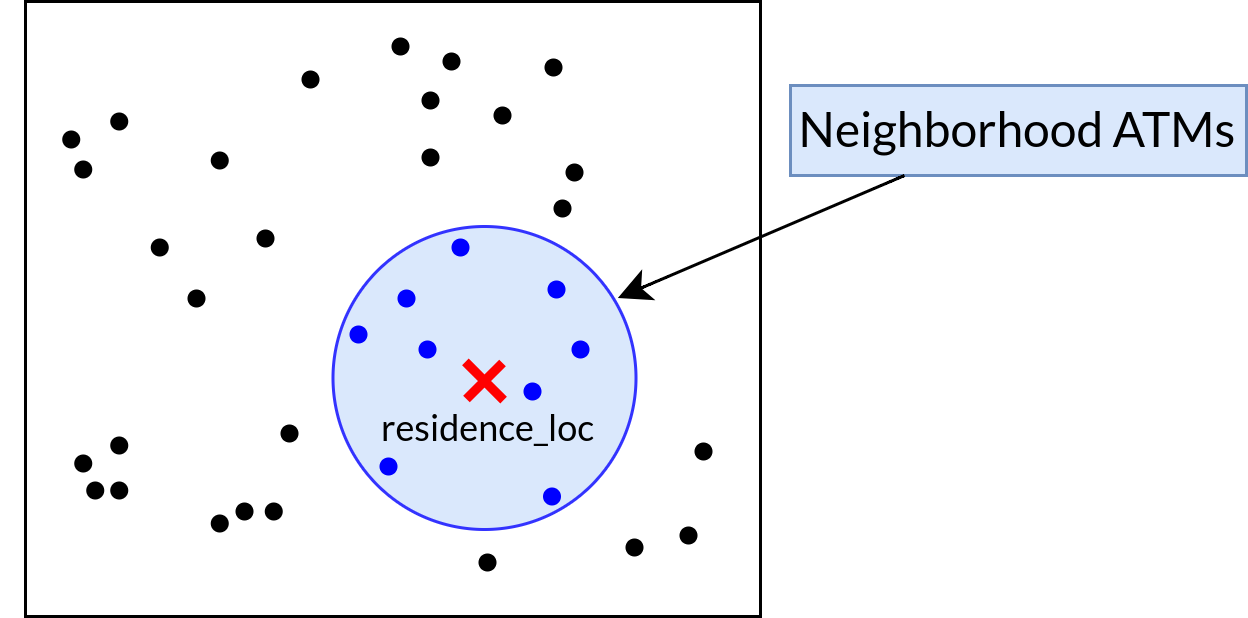
\includegraphics[scale=1.1]{images/tx-generation-1-named.png}
      \caption{\texttt{Neighborhood} ATM subset}
    \end{figure}

    \item \textbf{\texttt{t\_min}}: Minimum threshold time between any two consecutive 
    transactions of the client. That is, the minimum time distance between the end of 
    a transaction and the start of the next consecutive transaction of a card. 
    $$t_{min} = \frac{2 * \texttt{max\_distance}}{\texttt{max\_speed}}$$
    For the calculation of this minimum time distance:
    \begin{itemize}
      \item \texttt{max\_distance}: two options:  
        \begin{itemize}
          \item \textcolor{green}{$\Rightarrow$ DEFINETIVELY SELECT THIS, it is simpler and this way we give more margin to respect the min time and avoid undesired anomalous situations\\}In general: taking $2*\texttt{max\_distance}$ kms as the upper bound on 
          the maximum distance between 2 ATMs of the ATM subset, set the 
          \textcolor{orange}{\texttt{t\_min}} to be the time needed to traverse that distance 
          at a selected $\texttt{max\_speed}$. (* So far done like this). 
          \begin{figure}[H]
            \centering
            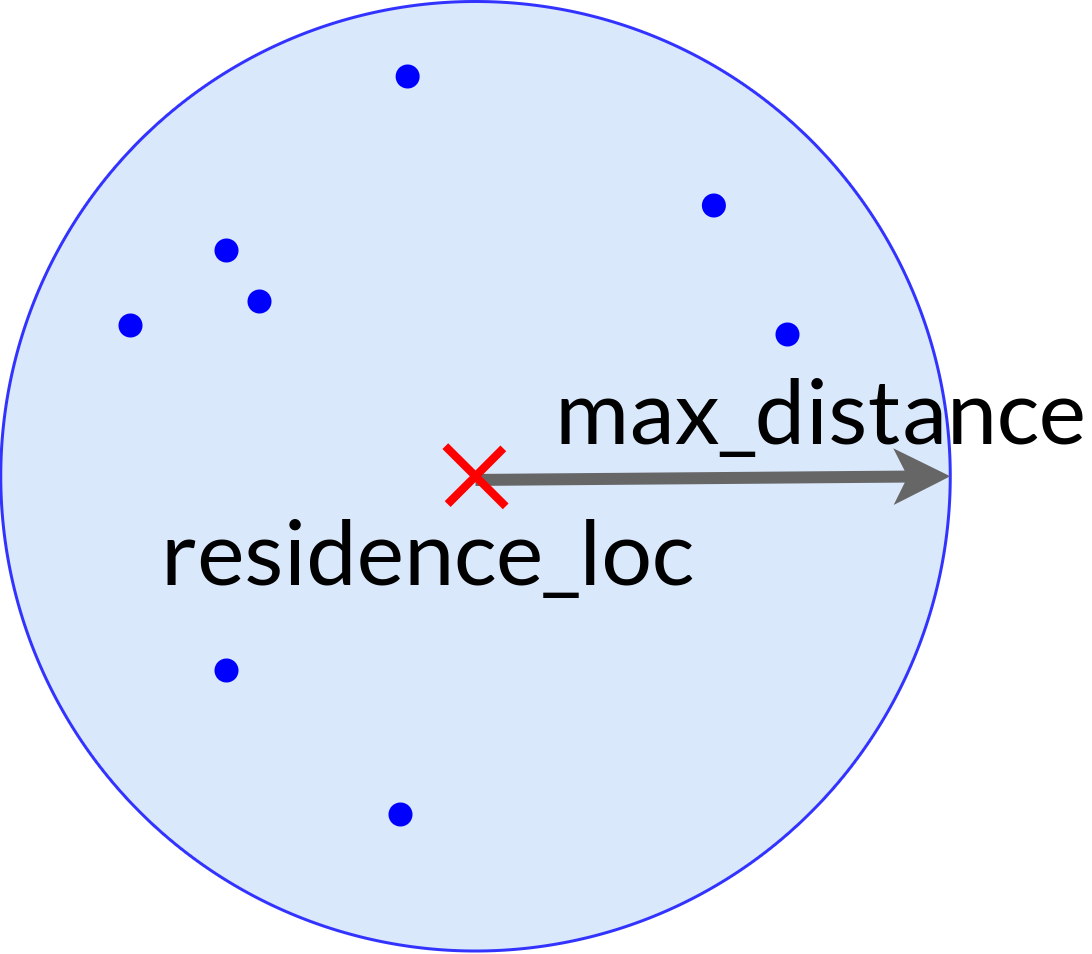
\includegraphics[scale=0.5]{images/tx-generation-tmin.png}
            \caption{\texttt{max\_distance} upper bound for the calculation of \texttt{t\_min}}
        \end{figure}    
          \item Specifically: Taking the specific maximum distance between all the ATM pairs 
          in the ATM subset to get the \textcolor{orange}{\texttt{t\_min}}.
      \end{itemize}  
      \item \texttt{max\_speed}: maximum speed at which it is possible to travel 
      (by any possible means of transport) between any pair of ATMs $\in 
      \ \texttt{Neighborhood}$.
    \end{itemize}

    \paragraph{NUMBER OF TX AND ITS DISTRIBUTION ALONG TIME:\\}
    \item \textcolor{red}{$\Rightarrow$ TODO: generate also other kinds of tx?} For each day generate \textcolor{orange}{\texttt{num\_tx}} transactions, random 
    number drawn from a Poisson distribution of $\lambda = \texttt{withdrawal\_day}$.

    \item \textcolor{red}{$\Rightarrow$ TODO: IMPROVE THE DISTRIBUTION ALONG TIME METHOD.
    Idea: do not do it by days, but for the time interval as a whole of the selected set of days!
    }Distribution of the \texttt{num\_tx} transaction times 
    (\texttt{transaction\_start}), doing a uniform distribution of the \texttt{num\_tx}
    for each of the days: 
    
    We create an ordered list of  \texttt{num\_tx} start moments in seconds in a day 
    (in the range $[\texttt{t\_min}/2, 86400-(\texttt{t\_min}/2)-\texttt{max\_duration}]$) so that all of them are at a minimum time distance of $\texttt{t\_min} + \texttt{max\_duration}$. See Figure \ref{img:tx-distribution}.
    \textit{\texttt{max\_duration} limits the maximum duration of an ordinary transaction. 
    For the moment it was set to be of 10 minutes (600s)}.\\
    Note that the interval bounds for the transaction start moments are designed in such 
    a way that the \texttt{t\_min} minimum time distance between the end of a transaction 
    and the start of the next transaction is also respected between transactions belonging 
    to different consecutive days. See Figure \ref{img:tx-distribution-day}. 
    \textcolor{red}{Note that this way of generation (day by day) we are not allowing 
    transactions to occur in the interval marked among the two red dotted lines of the 
    Figure \ref{img:tx-distribution-day}.} \textcolor{orange}{NOTE/TODO: This could be 
    fixed by looking to the start time of the last transaction of the previous day...}. 
    The start moments are therefore taken to define the \texttt{transaction\_start} of 
    each of the transactions of that day. \texttt{transaction\_end} is assigned a shifted 
    time difference with the respective \texttt{transaction\_start}, in particular the 
    difference is drawn from a normal distribution $\mathcal{N}(300,\,120)$ that defines 
    the duration of a transaction to be of mean of 5 minutes (300s) and a standard 
    deviation of 2 minutes (120s), bounding it to be of a maximum time of 
    \texttt{max\_duration} of 10 minutes (600s) and setting it to the mean if the 
    distribution sample was negative. 

    \begin{figure}[H]
        \centering
        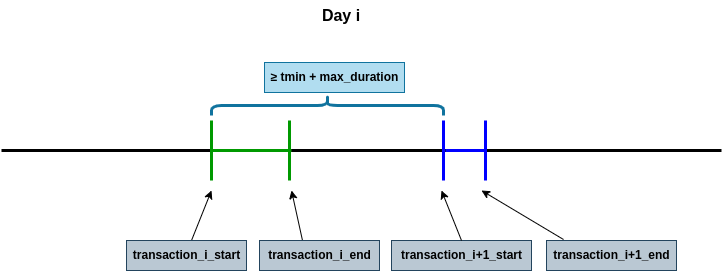
\includegraphics[scale = 0.45]{images/tx-distribution-1.png}
        \caption{Time distance limit between two consecutive transactions}
        \label{img:tx-distribution}
    \end{figure}
    \begin{figure}[H]
        \centering
        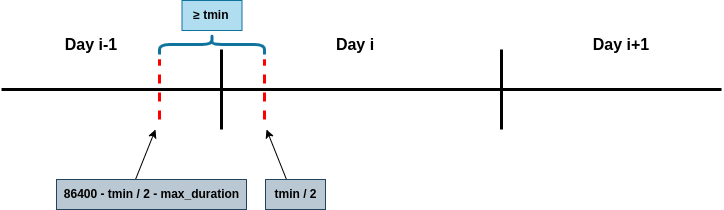
\includegraphics[scale = 0.45]{images/tx-distribution.png}
        \caption{Time distance limit between two consecutive transactions between two days}
        \label{img:tx-distribution-day}
    \end{figure}
    Note that a limit was set on the duration of the transaction so that we can have the 
    control avoiding time overlapping transactions, which will be producing irregular 
    undesired fraud pattern alerts.
    \item \texttt{transaction\_amount}: based on card behavior parameters, it is drawn 
    from a normal distribution
    $\mathcal{N}(\texttt{amount\_avg},\,\texttt{amount\_std})$. If negative amount, drawn 
    from a uniform distribution $\mathcal{U}(0,\ \texttt{amount\_avg}*2)$.
\end{itemize}

Note that this approach is done with the focus on avoiding the production of potential
fraud scenarios. By taking into account the previous generated transaction: both for the
linked ATM of the new transaction and its transaction time (to avoid transactions that 
are overlapped or that come one directly after the other, since this may be fraudulent!).

\subsubsection{ATM closed subset + Poisson Process}

\begin{tcolorbox}
  \begin{itemize}
    \item[$\rightarrow$] \textbf{ATM selection}: Closed ATM subset.
    \item[$\rightarrow$] \textbf{Time distribution}: Poisson process distribution of $num\_tx$ 
    transactions for each of the cards.
  \end{itemize}
\end{tcolorbox}

Generate $\texttt{num\_tx}$ transactions for a selected period of time $\texttt{t}$.
Distribution following a Poisson process distribution along $[0,t]$.
\begin{itemize}
    \item[$\bullet$] $\lambda=\texttt{avg\_tx}$ on a day for the client if $\texttt{t = 24h}$. Otherwise, 
    decide a specific $\lambda$ for the considered $\texttt{t}$.
    \item[$\bullet$] Inter-arrival times $X_1, X_2, \cdots$ are distributed following an exponential distribution:
    $X_i \sim \text{Exp}(\lambda)$. They represent the time elapsed between two of these events, e.g. $X_2$ represents the time elapsed between the first and the second arrival. Note that in this case, since we need to respect the minimum required time between two consecutive 
    transactions ($t_{min}$) so to avoid introducing anomalous undesired scenarios, we have to impose
    that: $X_i \geq \Delta_{i-1} + t_{min}, \forall X_i$, where:

    \begin{itemize}
      \item[$\circ$] $X_{i}$: time elapsed between the $i$-$1$ and $i$-th transaction.
      \item[$\circ$] $\Delta_{i-1}$: time duration of the $i$-$1$ transaction. This duration will 
      be upper bounded by $\Delta_{max}$, which will be considered the maximum possible duration of a transaction.
      \item[$\circ$] $t_{min}$: minimum calculated time distance between any 2 consecutive transactions of the client.
  \end{itemize}

    With these interarrival times, we obtain the arrival times $T_i$. Note that they are not independent, in particular:
    $T_1 \leq T_2 \leq T_3 \cdots$.

    Therefore, to generate the Poisson process with rate $\lambda$:
    \begin{enumerate}
      \item Generate i.i.d. random variables $X_1, X_2, \cdots$ where $X_i \sim \text{Exp}(\lambda)$.
      \item Obtain the arrival times as:
        \begin{itemize}
          \item $T_1 = X_1$
          \item $T_2 = X_1 + X_2$
          \item $T_3 = X_1 + X_2 + X_3$
          \item $\cdots$
        \end{itemize}
    \end{enumerate}

    Note that, having imposed the previous we will have that:
    \begin{equation}
      \begin{cases}
        T_i = T_{i-1} + X_i \\
        X_i \geq \Delta_{max} + t_{min}
      \end{cases}\forall X_i \
    \end{equation}

    which implies that:
    
    \begin{equation}
      T_i \geq T_{i-1} + \Delta_{max} + t_{min}, \forall X_i
    \end{equation}
    
\end{itemize}
\begin{figure}[H]
    \centering
    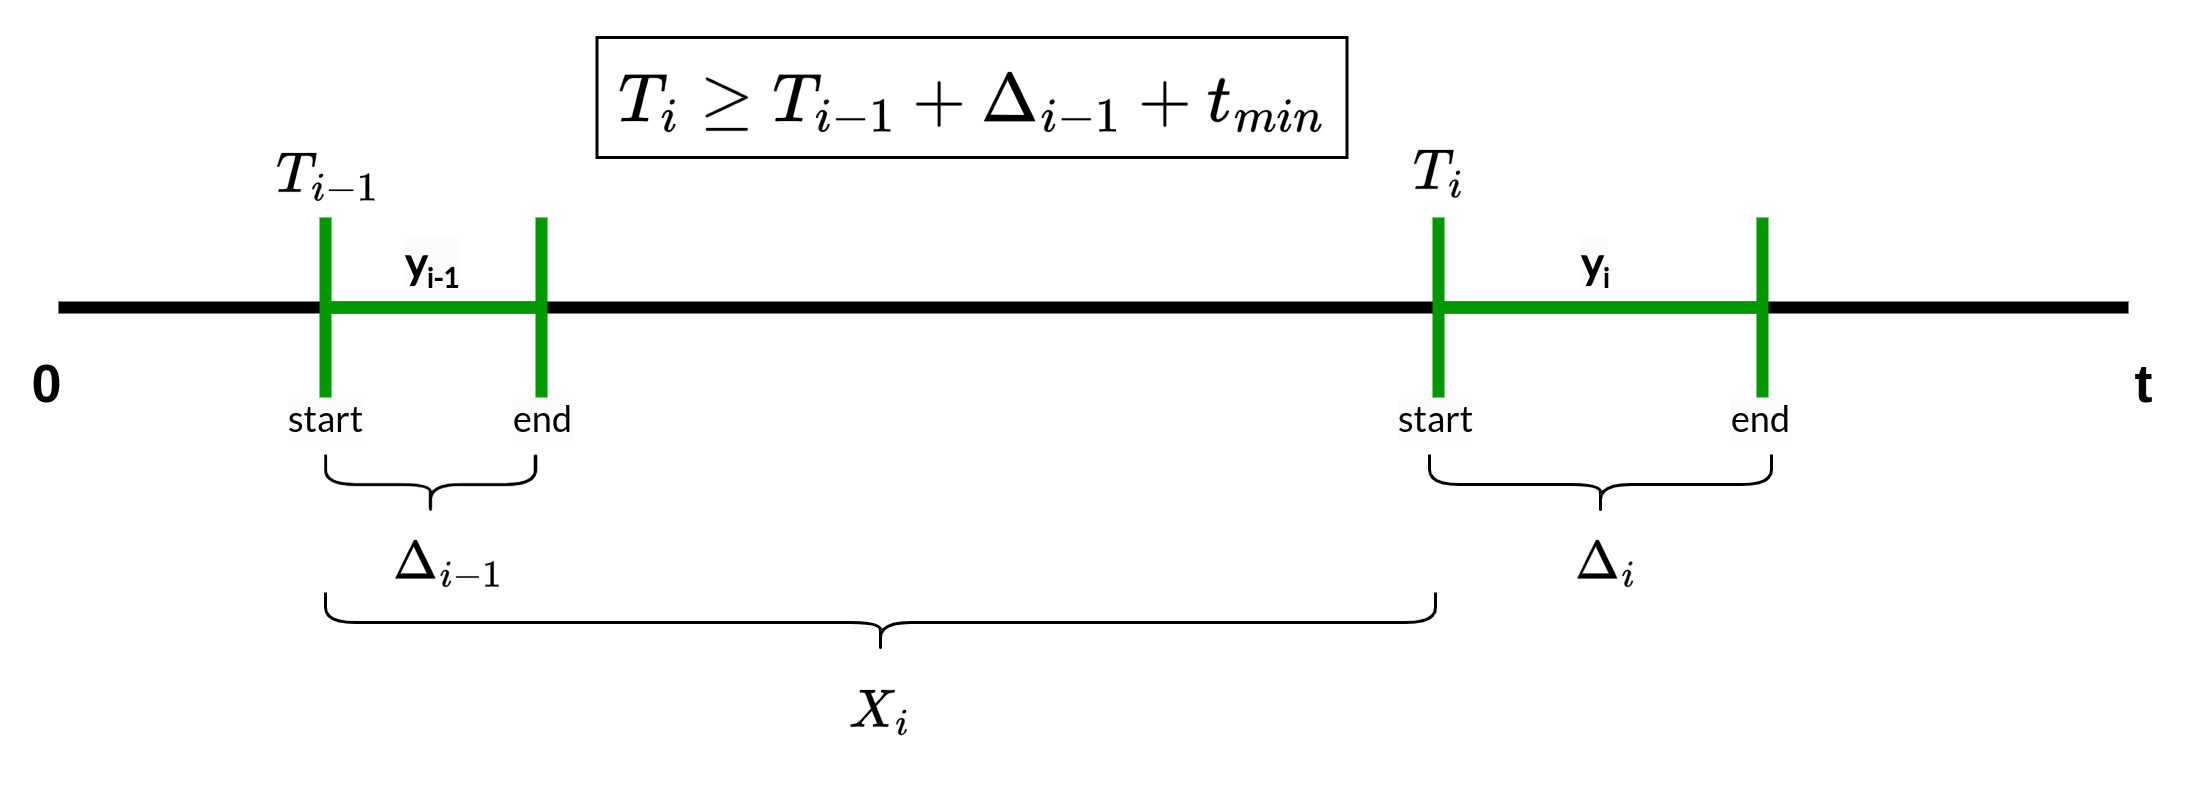
\includegraphics[scale=0.55]{images/tx-generation-dist-corrected.png}
    \caption{Schema of the interarrival and arrival event times on the poisson process.}
\end{figure}


References:

\begin{itemize}
  \item \href{https://www.probabilitycourse.com/chapter11/11_1_2_basic_concepts_of_the_poisson_process.php}{Poisson process modeling - Theoric description}
  \item \href{https://www.probabilitycourse.com/chapter14/Chapter_14.pdf}{Poisson process modeling - Python implementation}
  \item \href{https://timeseriesreasoning.com/contents/poisson-process/}{Less formal explanation with Python code}
  \item \href{https://www.math.wsu.edu/faculty/genz/416/lect/l05-45.pdf}{More theory}
  \item \href{https://en.wikipedia.org/wiki/Poisson_point_process}{Wikipedia entry}
\end{itemize}

\subsubsection{Random Walk / Markov Chain}

Idea is to model the sequence of transactions for each of the clients as a markov chain through the
network of ATMs. The network is a fully-connected graph with ATMs as nodes and edges are
weighted with the distance between each pair of ATMs as weights.

The idea is to obtain the sequence of transactions for each client as a markov chain, in which,
for each step a transaction is generated in that specific ATM node, at a certain datetime 
respecting the constraint of the minimum time distance with the previous transaction, so 
that no undesired anomalous fraud scenarios are produced. \\ 

Some considerations:
\begin{itemize}
  \item Initially, we will compute the transition matrix obtaining all the respective 
  transition probabilities. The probability of transition to another ATM-node will be 
  inversely proportional to the distance to the considered ATM-node.
  \item Transition matrix $P_t$: containing, for each state, the probability of transitioning
  between states. For example, the entry $i,j$: $(P_t)_{i,j} = \mathcal{P}(X_{t+1} = j | X_t = i)$
  contains the probability of transitioning to state $j$ when being in state $i$. 
  Note that since we assume a complete graph, and also the posibility to transition 
  to the same state, all entries of this matrix will be distinct to 0: $(P_t)_{i,j} \neq 0 \  
  \forall i,j$.
  \item Finally, once $P_t$ is computed, we perform the simulation to obtain the sequence of
  transactions for the specific card/client.
\end{itemize}

References:

\begin{itemize}
\item Markov Chains
\begin{itemize}
  \item \href{https://brilliant.org/wiki/markov-chains/}{MC - Theory}
  \item \href{https://www.columbia.edu/~ks20/4703-Sigman/4703-07-Notes-MC.pdf}{Simulation of Markov Chains - Theory}
  \item \href{https://stephens999.github.io/fiveMinuteStats/simulating_discrete_chains_1.html}{MC - Implementation example}
  \item \href{https://www.youtube.com/watch?v=G7FIQ9fXl6U}{MC - Implementation video example}
\end{itemize}
\item Random Walks
\begin{itemize}
  \item Theory:
  \begin{itemize}
    \item \href{https://ieeexplore.ieee.org/abstract/document/8911513?casa_token=vznpjKL5HG0AAAAA:hNzLCxAHBk75zCDUHsswB7ImAKgilzZcOBzxaXWz_G6U8Vy-ogbei40MoZ49M-Em5tTii0Q}{RWs: A Review of Algorithms and Applications}
    \item \href{https://www.lirmm.fr/~sau/JCALM/Josep.pdf}{RWs on Graphs}
    \item \href{https://www.fi.muni.cz/usr/gruska/random18/random1808.pdf}{RW - More theory}
  \end{itemize}
  \item Implementation examples:
  \begin{itemize}
    \item \href{https://tleise.people.amherst.edu/Math365Spring2016/RmarkdownFiles/WalkOnGraph.html}{Simple RW on a Graph - Implementation example}
    \item \href{https://graphstream-project.org/doc/Algorithms/Random-walks-on-graphs/}{A RW on a graph - Implementation}
    \item \href{https://es.mathworks.com/help/econ/simulate-random-walks-through-markov-chain.html}{Simulate Random Walks Through Markov Chain - Matlab Implementation example}
  \end{itemize}
\end{itemize}
\end{itemize}


\subsection{Population of the Graph Database}

% TODO: 
% 0. Description - Neo4j, what it is, why chosen...
% 1. Creation
% 2. Population

\subsubsection{Neo4j graph database creation}
% Neo4j Desktop y version - instalación y detalles. Cómo conectarse...
% TODO: Explain how to install / connect... all the details that are in the neo4.md file
\textcolor{red}{$\rightarrow$ TODO: 0. Describe on how to set up the database}
\textcolor{red}{$\rightarrow$ TODO: Explanation of the versions of both Neo4j instances used - local and UPC VM cluster.}\\

Prior to the population of the Neo4j graph database, a Neo4j graph database instance needs to be
created. This was done both locally and in a \textcolor{red}{Virtual Machine of the UPC cluster}.

Version: Neo4j 5.21.0 Community edition. 
\begin{itemize}
    \item Accessing it: by default it runs on localhost port 7474: \texttt{http://localhost:7474}.
    Start the neo4j service locally by: \texttt{sudo systemctl start neo4j}\\
    It can be also be accessed by the internal utility \texttt{cypher-shell}. Username: \texttt{neo4j} and password: \texttt{bisaurin}.
\end{itemize}

\subsubsection{Neo4j graph database population - CSV to PG}
\begin{comment}
    - Creación de la GDB - de CSV a Neo4j PG: 
    - Poner primero los comandos cypher por separado, con las constraints de uniqueness
    y luego lo de poblar. Luego ya referir a que todo ello se tiene en un único script que 
    permite la ejecución directa (en lugar de paso a paso) en golang.
    - Incluir detalles específicos de cada CSV...
\end{comment}

Once we created the Neo4j graph database instance and all the CSV data files representing all the nodes and relations, we populate the Property Graph instance in Neo4j. Before performing the population of the GDB, we create uniqueness constraints on the properties of the nodes that we use as our \emph{de facto} IDs for the ATM and Card IDs: \texttt{ATM\_id} and \texttt{number\_id}, respectively. The reason to do this is to avoid having duplicated nodes of these types with the same ID in the database. Therefore, as an example, when adding a new ATM node that has the same \texttt{ATM\_id} as another ATM already existing in the database, we are aware of this and we do not let this insertion to happen. ID uniqueness constraints are created with the following cypher directives:

\begin{center}
\lstset{style=cypherStyle}
\begin{lstlisting}[caption={Uniqueness ID constraints}]
            CREATE CONSTRAINT ATM_id IF NOT EXISTS
            FOR (a:ATM) REQUIRE a.ATM_id IS UNIQUE
    
            CREATE CONSTRAINT number_id IF NOT EXISTS
            FOR (c:Card) REQUIRE c.number_id IS UNIQUE
    
            CREATE CONSTRAINT code IF NOT EXISTS
            FOR (b:Bank) REQUIRE b.code IS UNIQUE
\end{lstlisting}
\end{center}

Once we created the Neo4j graph database instance and all the CSV data files representing all the nodes and relations, we populate the Property Graph instance in Neo4j. For this, we propose two different methods. The first does it by directly importing the CSV files using the Cypher's \texttt{LOAD CSV} command, while the second method does it by parsing the CSV data and running the creation of the nodes and relationships using Cypher. Both methods can be found and employed using the \texttt{populatemodule} golang module.
In this module we can find the two subdirectories where each of the methods can be run. In detail, the module tree structure is depicted in Figure \ref{fig:populatemodule}. On it, the \texttt{cmd} subdirectory contains the scripts to run each of the populating methods: the first method script on \texttt{csvimport} and the second on the \texttt{cypherimport}, while the \texttt{internal} subdirectory is a library of the files with the specific functions used by these methods.

\begin{figure}[h]
\centering
\begin{forest}
  for tree={
      font=\ttfamily,              % Typewriter font for file names
      grow'=0,                      % Tree direction (left-to-right)
      child anchor=west,            % Children alignment
      parent anchor=east,           % Parent alignment
      anchor=west,                  % Tree alignment
      calign=first,                 % Aligns with the first child
      edge path={
          \noexpand\path [draw, thick, \forestoption{edge}] (!u.parent anchor) -- +(-1pt,0) |- (.child anchor)\forestoption{edge label};
      },
      inner sep=4pt,
      l=10pt,                       % Level distance
      s sep=5pt                     % Sibling distance
  }
  [populatemodule
      [cmd
        [csvimport
            [main.go]
            [.env]
        ]
        [cypherimport
            [main.go]
            [.env]
        ]
      ]
      [internal
          [common
              [common.go]
          ]
          [populate
              [populate.go]
          ]
      ]
  ]
\end{forest}
\caption{\texttt{populatemodule} file structure}
\label{fig:populatemodule}
\end{figure}

% How to run it - .env file
% Description of each of the methods


Prior to run any of these methods we need to first set up correctly the \texttt{.env} file located inside the desired method directory, where we have to define the corresponding Neo4j URI, username and password to access the Neo4j graph database instance.

\begin{itemize}
\item{\textbf{Method 1: Cypher's \texttt{LOAD CSV}}\\}
The Cypher's \texttt{LOAD CSV} clause allows to load CSV into Neo4j, creating the nodes and relations expressed on the CSV files (see \href{https://neo4j.com/docs/cypher-manual/5/clauses/load-csv/}{\textit{load-csv cypher manual}}). 
To use it simply follow these steps:
\begin{enumerate}
    \item Place all the CSVs (\texttt{atm.csv}, \texttt{bank.csv}, \texttt{card.csv}, \texttt{atm-bank-internal.csv}, \texttt{atm-bank-external.csv} 
    and \texttt{card-bank.csv}) under the \texttt{/var/lib/neo4j/import} directory
    of the machine containing the Neo4j graph database instance.
    \item Run \texttt{\$ go run populatemodule/cmd/csvimport/main.go}
\end{enumerate}

\paragraph{Process description:}

Then the different CSV files containing all the data tables of our data set, were loaded into the GDB with the following cypher directives.

% TODO: Esto es en mi local. Se recomienda por razones de seguridad... Sin embargo se puede configurar para que no sea
% así. - En el cluster veremos. De momento no pongo nada de esto!
% First, the CSV files were needed to be placed under the \texttt{/var/lib/neo4j/import} directory.

\paragraph{ATM (atm.csv)}

\begin{center}
\lstset{style=cypherStyle}
\begin{lstlisting}[caption={atm.csv}]
    LOAD CSV WITH HEADERS FROM 'file:///csv/atm.csv' AS row
    MERGE (a:ATM {
        ATM_id: row.ATM_id,
        loc_latitude: toFloat(row.loc_latitude),
        loc_longitude: toFloat(row.loc_longitude),
        city: row.city,
        country: row.country
    });
\end{lstlisting}
\end{center}

Some remarks:
\begin{itemize}
    \item \texttt{ATM} is the node label, the rest are the properties of this kind of node.
    \item Latitude and longitude are stored as float values; note that they could also be stored
    as cypher \textit{Point} data type. However for the moment it is left like this. In the future
    it could be converted when querying or directly be set as cypher point data type as property.
\end{itemize}

\paragraph{Bank (bank.csv)}

\begin{center}
\lstset{style=cypherStyle}
\begin{lstlisting}[caption={bank.csv}]
    LOAD CSV WITH HEADERS FROM 'file:///csv/bank.csv' AS row
    MERGE (b:Bank {
        name: row.name, 
        code: row.code, 
        loc_latitude: toFloat(row.loc_latitude), 
        loc_longitude: toFloat(row.loc_longitude)
    });
\end{lstlisting}
\end{center}

Note that the \texttt{code} is stored as a string and not as an integer, since to make it more clear it 
was already generated as a string code name.

\paragraph{ATM-Bank relationships (atm-bank-internal.csv and atm-bank-external.csv)}

\begin{center}
\lstset{style=cypherStyle}
\begin{lstlisting}[caption={atm-bank-internal.csv}]
    LOAD CSV WITH HEADERS FROM 'file:///csv/atm-bank-internal.csv' AS row
    MATCH (a:ATM {ATM_id: row.ATM_id})
    MATCH (b:Bank {code: row.code})
    MERGE (a)-[r:BELONGS_TO]->(b);
\end{lstlisting}
\end{center}

\begin{center}
\lstset{style=cypherStyle}
\begin{lstlisting}[caption={atm-bank-external.csv}]
    LOAD CSV WITH HEADERS FROM 'file:///csv/atm-bank-external.csv' AS row
    MATCH (a:ATM {ATM_id: row.ATM_id})
    MATCH (b:Bank {code: row.code})
    MERGE (a)-[r:INTERBANK]->(b);
\end{lstlisting}
\end{center}

\paragraph{Card (card.csv)}

\begin{center}
\lstset{style=cypherStyle}
\begin{lstlisting}[caption={card.csv}]
    LOAD CSV WITH HEADERS FROM 'file:///csv/card.csv' AS row
    MERGE (c:Card {
        number_id: row.number_id, 
        client_id: row.client_id, 
        expiration: date(row.expiration), 
        CVC: toInteger(row.CVC), 
        extract_limit: toFloat(row.extract_limit), 
        loc_latitude: toFloat(row.loc_latitude), 
        loc_longitude: toFloat(row.loc_longitude)});
\end{lstlisting}
\end{center}

Notes:
\begin{itemize}
    \item We do not include the fields that were generated to define the behavior of the card. They are only used for the generation of the transactions.
    \item \texttt{expiration}: set as \textit{date} data type.
\end{itemize}

\paragraph{Card-Bank relationships (card-bank.csv)}

\begin{center}
\lstset{style=cypherStyle}
\begin{lstlisting}[caption={card-bank.csv}]
    LOAD CSV WITH HEADERS FROM 'file:///csv/card-bank.csv' AS row
    MATCH (c:Card {number_id: row.number_id})
    MATCH (b:Bank {code: row.code})
    MERGE (c)-[r:ISSUED_BY]->(b);
\end{lstlisting}
\end{center}

%\subsubsection*{Dataset extensions}

\begin{comment}
- Interesting reference for coordinates and distances in cypher - https://lyonwj.com/blog/spatial-cypher-cheat-sheet 
- Transactions dataset Generation  - a transaction dataset simulator → useful with the description of fraud scenarios, that can be generated among the transactions dataset, also with customers and terminals info generation (similar to ATMs concept) 
\end{comment}

\item Method 2:

\end{itemize}

\textcolor{red}{$\rightarrow$ TODO: Describe the other population method}

\textcolor{green}{\rule{\linewidth}{0.4mm}}


\section{Indexing}

Useful for ensuring efficient lookups and obtaining a better performance as the database 
scales.

$\rightarrow$ indexes will be created on those properties of the entities on which the 
lookups are going to be mostly performed; specifically in our case:
\begin{itemize}
  \item Bank: \texttt{code} ?
  \item ATM: \texttt{ATM\_id}
  \item Card: \texttt{number\_id}
\end{itemize}

Why on these ones?

$\rightarrow$ Basically the volatile relations / transactions only contain this information,
which is the minimal information to define the transaction. This is the only information that
the engine recieves from a transaction, and it is the one used to retrieve additional information - the complete information details of the ATM and Card nodes on the complete
stable bank database. Therefore these parameters/fields (look for the specific correct
word on the PG world) are the ones used to retrieve / query the PG. 

By indexing or applying a unique constraint on the node properties, queries related to these entities can be optimized, ensuring efficient lookups and better performance as the database scales.

From Neo4j documentation:
\begin{tcolorbox}
  An index is a copy of specified primary data in a Neo4j database, such as nodes, relationships, or properties. The data stored in the index provides an access path to the data in the primary storage and allows users to evaluate query filters more efficiently (and, in some cases, semantically interpret query filters). In short, much like indexes in a book, their function in a Neo4j graph database is to make data retrieval more efficient.
\end{tcolorbox}

Some references on indexing:
\begin{itemize}
  \item \href{https://neo4j.com/docs/cypher-manual/current/indexes/search-performance-indexes/overview/}{Search-performance indexes}
  \item \href{https://neo4j.com/docs/cypher-manual/current/indexes/search-performance-indexes/using-indexes/}{The impact of indexes on query performance}
  \item \href{https://neo4j.com/docs/cypher-manual/current/indexes/search-performance-indexes/managing-indexes/}{Create, show, and delete indexes}
\end{itemize}

Okay... but before diving deeper...:

\textbf{To Index or Not to Index?}
\begin{tcolorbox}
When Neo4j creates an index, it creates a redundant copy of the data in the database. Therefore using an index will result in more disk space being utilized, plus slower writes to the disk.

Therefore, you need to weigh up these factors when deciding which data/properties to index.

Generally, it's a good idea to create an index when you know there's going to be a lot of data on certain nodes. Also, if you find queries are taking too long to return, adding an index may help.
\end{tcolorbox}

From \href{https://www.quackit.com/neo4j/tutorial/neo4j_create_an_index_using_cypher.cfm#google_vignette}{another tutorial on indexing in neo4j}\\

$\rightarrow$ Apparently, there are \emph{Token lookup indexes} which are a default type of node indexes, from the Neo4j documentation: \textit{"Two token lookup indexes are created by default when creating a Neo4j database (one node label lookup index and one relationship type lookup index). Only one node label and one relationship type lookup index can exist at the same time."}. 
That is, two indexes are created by default, they are on the node label and on the relationship type.\\

$\rightarrow$ There are different type of indexes depending on what we want to use them for, the type of property that they index...: \href{https://neo4j.com/docs/cypher-manual/current/indexes/search-performance-indexes/managing-indexes/#create-indexes}{see here for more details.}\\

$\rightarrow$ An example on when to use indexes: \href{https://stackoverflow.com/questions/51313374/what-is-indexing-means-neo4j-and-how-it-effects-performance}{example case}.\\



\textcolor{green}{$\rightarrow$ \textbf{Decision}: Create indexes on the ATM and Card node properties which serve as our node identifiers in practice: on \texttt{ATM\_id} and on \texttt{number\_id} node properties.} The reason is that, so far, most of the queries are performed looking at a single node using its identifier; in particular to retrieve ATM nodes location coordinates to calculate the distance between two ATM nodes.\\
\textcolor{red}{POSSIBLE IMPROVEMENT $\rightarrow$ make Neo4j obtain/calculate/return this distance as the result of a query.}


\paragraph{Description of the creation on indexes\\}

\begin{enumerate}
  \item Select the type of index: range index VS text index\dots
  Some references on this election:
  \begin{itemize}
    \item \href{https://stackoverflow.com/questions/77833955/neo4j-range-index-vs-text-index-when-checking-membership-in-list-of-only-strin}{Use range index (the default), if we do not need to use
    \texttt{CONTAINS}, \texttt{ENDS WITH} or the value size is not above
    8k}.
  \end{itemize}
  \item Note that for the text index we (may) need to guarantee that the property type is STRING: \href{https://neo4j.com/docs/cypher-manual/current/constraints/managing-constraints/#create-single-property-type-constraint}{create a single property type constraint}.
\end{enumerate}

\bibliographystyle{plain} % Choose a style (plain, abbrv, unsrt, etc.)
\bibliography{references} % This points to references.bib

\end{document}